
\documentclass[chapter,11pt,oneside,openany]{xoblivoir}

% \pagestyle{hangul}

% \usepackage{draftwatermark}
% \SetWatermarkLightness{0.9}

\usepackage{subfig}
\usepackage{amsmath}
\usepackage{graphicx}

\usepackage{fapapersize}
\usefapapersize{210mm,290mm,30mm,*,35mm,30mm}

% HY신명조
\setkormainfont(-윤명조340)(*){-윤명조320}

\hypersetup{pdfborder={0 0 0}}

\SetHangulspace{1.6}{1.2}
%\renewcommand{\baselinestretch}{1.6}

% \setcounter{tocdepth}{3}
% \setcounter{secnumdepth}{3}
% \newcounter{APPsubsubsection}

\maxsecnumdepth{subsubsection}

\renewcommand\thesection{\arabic{chapter}.\arabic{section}}
\renewcommand\thesubsection{\thesection.\gana{subsection}}
\renewcommand\thesubsubsection{\thesubsection.\arabic{subsubsection})}

\usepackage[noindentafter]{titlesec}

\titleformat{\chapter}{\huge\bfseries\centering\vspace{-80pt}}{제\thechapter장}{20pt}{}[\vspace{-30pt}]
\titleformat{\section}{\Large\bfseries}{\thesection.}{13pt}{}[\vspace{-7pt}]
\titleformat{\subsection}{\large\bfseries}{\hspace{11pt}\thesubsection.}{13pt}{}[\vspace{-7pt}]
\titleformat{\subsubsection}{\bfseries}{\hspace{22pt}\thesubsubsection}{13pt}{}[\vspace{-7pt}]

\renewcommand\cftsectionindent{1.0em}
\renewcommand\cftsectionnumwidth{2.5em}
\renewcommand\cftsubsectionindent{3.0em}
\renewcommand\cftsubsectionnumwidth{3.5em}

\usepackage{wallpaper}

\title{화분을 구별할 수 있는 물 분사 시스템}
\author{와룡고등학교 2학년 류형욱}
% \date{\today}

\begin{document}

\pagestyle{plain}

\frontmatter
\ThisCenterWallPaper{}{img/title}

%%
 %
%%

\newpage

% \maketitle
% \begin{abstract}
% 인식표만 부착하면 영상처리 알고리즘을 이용하여 특정 위치에 자동으로 물을 뿌릴 수 있으며 로컬 또는 원격에서 실시간 수동제어도 가능한 작품
% \end{abstract}

\tableofcontents
\listoffigures
\listoftables

\mainmatter

\chapter{제작 동기와 목적}

\section{제작 동기}

우리 반 교실 창틀과 교탁 위에는 학생들이 가져온 화분이 많다.
학기 초에 한 학생이 화분을 가져왔는데, 삭막한 교실이 환해져서인지
다른 반 학생과 선생님들의 반응이 의외로 좋았다.
그 때부터 하나 둘 가져오기 시작한 것이 지금은 수십 개에 달한다.

나는 한 학기 동안 이 화분 관리를 담당하게 되었다.
식물마다 제각기 다른 관수 주기를 만족시키기 위해
처음에는 교실 벽면의 화이트보드에 화분의 이름과 다음 관수일을 기록하는 방법으로
화분을 관리하였지만, 화분의 수가 많아지자 관수 주기를 일일히 적어서
관리하기가 어렵고 귀찮아 물을 주는 시기를 놓치는 때도 종종 있었다.

누가 화분을 대신 관리해 주면 좋겠다는 생각을 하던 중
타이머나 간단한 자동 제어로 특정 시간 간격으로
물을 분사하는 시스템이 있으면 가능할 것 같았다.
평소에 정보 기기에 대해 관심이 많았기 때문에 이를 한 번 만들고 싶은 생각이
들었다. 그러나 단순히 `이틀에 한 번', `일주일에 한 번' 하는 식으로 단순하게
물을 주기 보다 뭔가 특별한 기능을 하는 물 분사 시스템을 만들어 보고 싶어졌다.
만약 주기적으로 물만 분사되는 시스템이라면
누군가가 임의로 화분을 이동시켰을 때 화분에 물을 정확히 뿌리지 못하고
교실이 물바다가 될 것 같았다.

이에 화분이 예기치 않게 이동되어도 화분의 위치를 찾아서 식물의 종류를 인식하고
스스로 물을 뿌리는 시스템이라면 이런 문제를 해결할 수 있다고 보고,
화분을 구별하는 물 분사 시스템을 제작하게 되었다.

\section{제작 목적}

\subsection{사용자 개입 없이 자동으로 화분을 구별할 수 있다.}
\label{autoDetect}
직접 개발한 영상 처리 알고리즘\footnote{AForge.NET Framework 기반}을 사용하여 카메라에서 얻은 화상에서
화분에 부착된 마커를 추출하고 마커의 종류를 인식함으로써 화분을 구별한다.


\subsection{예기치 못한 화분 위치 이동에도 문제 없이 화분을 인식한다.}
미리 좌표를 지정하지 않고 매번 전 구역에 대해 영상 처리를 수행하고 화분에 부착된 마커를 인식하게 하여
사용자가 화분을 옮겨도 마커 추적을 통해 화분을 인식한다,

\subsection{계획에 따라 스스로 물을 뿌릴 수 있다.}
화분의 종류에 따라 관수 주기와 양을 등록해 놓아 영상 처리 정보만 입력되면
\ref{autoDetect}에 따라 살수를 수행하도록 한다.

\subsection{사용자가 개입하여 실시간 제어할 수 있다.}
사용자가 직접 제어를 원할 경우 시스템의 높은 확장성을 이용해
실시간 제어를 가능하게 한다.

\subsection{부착된 마커를 인식하여 특정 범위에 물을 분사할 수 있다.}
마커를 읽어 물을 분사하는 시스템의 기본 사양을 활용,
이를 자동 범위 청소와 같은 여러 분야에 응용 한다.


\chapter{작품의 내용}

\section{작품 구성}

작품의 구성 요소를 논리적 기능으로 분류하면 호스트 시스템, 임베디드 시스템,
물리 장치와 같이 세 부분으로 나눌 수 있다. 또 호스트 시스템을 상위 계층으로,
임베디드 시스템과 물리 장치를 하위 계층으로 나눌 수 있다.

이 절에서는 작품 구성 요소가 수행하는 기능을 중심으로 작품을 설명한다.

\subsection{임베디드 시스템}

\subsubsection{MCU}
임베디드 시스템을 제어하는 CPU로서 ATmega128A를 사용한다.
임베디드 시스템은 호스트 시스템의 명령을 받아 동작하며, 카메라와 노즐의 상하 방향과 좌우 방향을 제어하는 모터와,
펌프와 밸브의 켜짐 또는 꺼짐 상태를 제어한다.
명령을 받고 제어를 수행하기 위해 임베디드 시스템과 호스트 시스템은 USB로 연결되어 시스템이 작동되는 동안 계속 통신을 수행한다.

\subsubsection{통신}
제어를 위해 PC와 MCU는 양방향으로 통신을 수행한다.
임베디드 시스템은 초기화 작업을 수행한 뒤 곧바로 통신 루틴으로 진입하고,
PC에서 전송되는 데이터를 폴링하면서 새로운 패킷을 계속 받는다. 완성된 패킷이 도착하면 해당하는 서비스 루틴을 실행한다.
임베디드 시스템이 명령을 받아 처리할 수 있는 작업에는
정상 작동 여부 확인, 비상 정지, 팬 스텝 입력, 틸트 폭 입력, 펌프 켜기 / 끄기가 있다.

끊김 없는 부드러운 제어를 실현하고 마커 인식률을 높이기 위해
모터를 제어하는 데 있어 지연을 줄일 수 있는 통신 방법이 필요하다.
호스트 시스템은 임베디드 시스템에 명령을 보낼 때 값을 직접 전송하지 않고
이동 방향과 변화량만 전송한다. PC에서는 임베디드 시스템의 특정 변수가 목표치에
도달할 때까지 계속 현재 상태를 요청하고, 목표치에 도달하면 중지 명령을 보낸다.
이러한 방법은 복잡하게 구현되지만 두 시스템 사이에서 발생되는 지연을 사용자가
거의 알아차릴 수 없게 만든다.


\subsection{물리 장치}

\subsubsection{전원}
모터나 펌프, 밸브와 같은 부하는 MCU(마이크로 프로세서)의 불안정을
초래할 수 있기 때문에 포토 커플러를 이용해 모터 전원과 시그널 전원을
분리하고 있다.

\subsubsection{구동 장치}
시스템은 바닥에 고정된 상태로 운용되며, 필요한 경우 사용자가 시스템을 중지하고 직접 이동해야 한다.
고정된 상태에서 주변의 마커를 인식하고 살수하기 위해서는 카메라와 노즐이 상하 좌우로 움직일 수 있어야 하는데,
작품에서는 팬 제어(좌우 제어)에 스테핑 모터, 틸트 제어(상하 제어)에 서보 모터를 사용한다.

\subsubsection{수압 장치}
장치에서 수압을 얻는 부분은 펌프와 밸브로 구성된다.
임베디드 시스템은 릴레이를 제어하여 수압 계통의 펌프와 밸브를
켜거나 끈다.

시스템을 대규모로 만들 경우에는 수돗물과 같이 외부에서 물을 공급받으면
현재 보다 훨씬 더 안정적인 살수가 가능할 것이다.

\subsubsection{살수 역학}
\label{water}

작품을 개발하는 동안 많은 실험과 설계 변경이 살수 기능을 구현을 위해 이루어졌다.
아래 몇 가지는 살수 기능을 구현하기 위한 간단한 이론적 배경이다.

저항을 받지 않는 포물체의 좌표를 $(x, y)$, 초기 속력을 $v_0$,
노즐과 바닥 사이의 각도를 $\theta$라 하면, 시간 $t$일 때
물체의 위치는 다음과 같이 주어진다.
\begin{equation}
\label{eq:x}
x = v_0 cos \theta t
\end{equation}
\vspace{-10mm}
\begin{equation}
\label{eq:y}
y = v_0 sin \theta \cdot t - \frac{1}{2}gt^2
\end{equation}
여기에서 식 \eqref{eq:y}은 노즐에서 나온 물이 살수 목표에 다다르기까지
계속 연직 하방으로 가속되며, 노즐의 방향이 곧장 살수 목표를 향하게 되면
물줄기는 살수 목표에 다다르지 못함을 보여준다.

식 \eqref{eq:x}와 식 \eqref{eq:y}는 실질적인 물의 운동을 설명하지 못하는데,
여러 저항이 존재한다는 것과 유체의 특성이 반영되지 못했기 때문이다.
그 이유에는 여러 가지가 존재한다.
\begin{itemize}
\item 펌프에 일정한 저항이 작용하고, 안정된 전력을 인가하여도
임펠러의 분당 회전수가 정확히 고정되지 않는 특성이 있다.
따라서 노즐에서 토출되는 물의 속도 $v_0$을 일정하게 얻을 수 없다.

\item 노즐의 상하 각도가 높아지면 물통 수면에 대한 노즐 끝의 높이도 높아지며,
펌프 작동에 저항하는 압력도 커진다. 그런데 펌프의 출력이 저항에 대해
선형적이지 않기 때문에 펌프에 가해지는 저항에 따른 토출수의 속력을
쉽게 예측할 수 없다.
\end{itemize}
그렇기 때문에 두 식이 살수되는 물의 운동을 파악하는 데
실질적인 도움은 되지 못하지만, 적어도 살수를 구현하는 데 있어서 더 복잡한 방법이
필요함을 보인다.

작품에서는 보다 더 공학적인 관점으로 접근하여, 포물선으로 살수할 때 몇 가지 각도에 따른 적합한 살수 목표의 거리와 높이를 실험적으로 구해 미리 입력해두는 방법을 사용한다.
살수 기능이 실제로 동작할 때는 목표의 거리와 높이를 구한 상태에서,
살수하기 직전 실행 시간에 보간법을 사용해 적절한 각도를 구해낸다.


\subsubsection{카메라}
\label{cam}
화상을 얻기 위해 USB 웹캠을 사용한다. 화상은 실시간으로 호스트 시스템에 직접 전송된다. 표준을 따르는 이미징 장치는 모두 카메라로 사용할 수 있고, 테스트를 위해서는
정지 영상도 처리가 가능하다.

좌우 방향 제어는 카메라와 노즐이 동시에 이루어지지만, 상하 방향 제어는 카메라와 노즐이 독립적으로 구성되어 있다.

화분에 살수할 때, 살수된 물이 지면과 이루는 각은 클수록 좋은데,
각이 너무 작으면 화분에 담긴 흙이 주위로 튀기 때문이다.
짧은 거리에 위치한 화분에 큰 각도로 살수하기 위해서는 살수된 물이
포물선의 궤적을 그리도록 해야 하고, \ref{water}에 따라 노즐이 큰 각도로
설정되어야 한다.

그런데, 카메라와 노즐이 같은 상하 방향 제어를 공유하면 포물선 살수를 진행 하는
동안 카메라는 `허공'을 바라보게 되어 아무런 작업도 수행할 수 없게 된다.
상하 제어에 필요한 시간도 한정된 자원이므로 허공을 바라보는 카메라의
각도를 다시 줄이는 작업이 오버헤드로 작용하고, 결국 장치의 이용률에
나쁜 영향을 미치게 된다.

어떤 방법을 사용하는 경우라도 살수하는 동안에는 물줄기가 인식을 방해하므로
영상 처리를 진행할 수 없다. 하지만 카메라와 노즐의 상하 방향 제어를
독립적으로 수행하면 포물선 살수 이후 탐색 상태로 전환하는 데
물리적인 이동 과정이 요구되지 않으므로
마커 인식과 살수 작업을 끊김 없이 반복 수행할 수 있다는 장점이 있다.


\subsection{호스트 시스템}

\subsubsection{소프트웨어 구성}
소프트웨어는 현재 로컬에서만 사용할 수 있으며,
관리자(Manager), 스케줄러(Scheduler), 영상 처리기(ImageProcessor), 문맥(Context),
물리 장치(PhysicalDevice), 마커(Marker), 식물(Plant)과 같은 여러 클래스(모듈)로 구성되어있다.


\subsubsection{플랫폼}
작품 전체에서 사용할 수 있는 플랫폼은 Microsoft Windows XP, Windows 7 뿐이다.
하지만 추후 시스템의 규모를 확대하고 `서버 - 클라이언트' 구조를 도입할 경우에는
스마트폰과 웹 표준을 지원하는 많은 브라우저에서 시스템에 접근할 수 있을 것이다.
또 웹뿐만 아니라 상호 운용성(Interoperability)이 높은 인터페이스를 노출하면
다양한 기기에 대한 네이티브 클라이언트도 개발할 수 있다.

\subsubsection{영상 처리 모듈}
영상 처리 기술은 호스트 시스템이 물리 장치의 상태를 파악할 수 있게 하는 아주 중요한 부분이다.
카메라는 호스트 시스템에 직접 연결되고, 영상 처리 모듈이 카메라의 화상을 받아 영상을 처리한다.

\subsubsection{마커}
\label{marker}

\begin{figure}[ht]
\centering

\includegraphics[width=0.17\textwidth]{img/red}

\includegraphics[width=0.17\textwidth]{img/green}
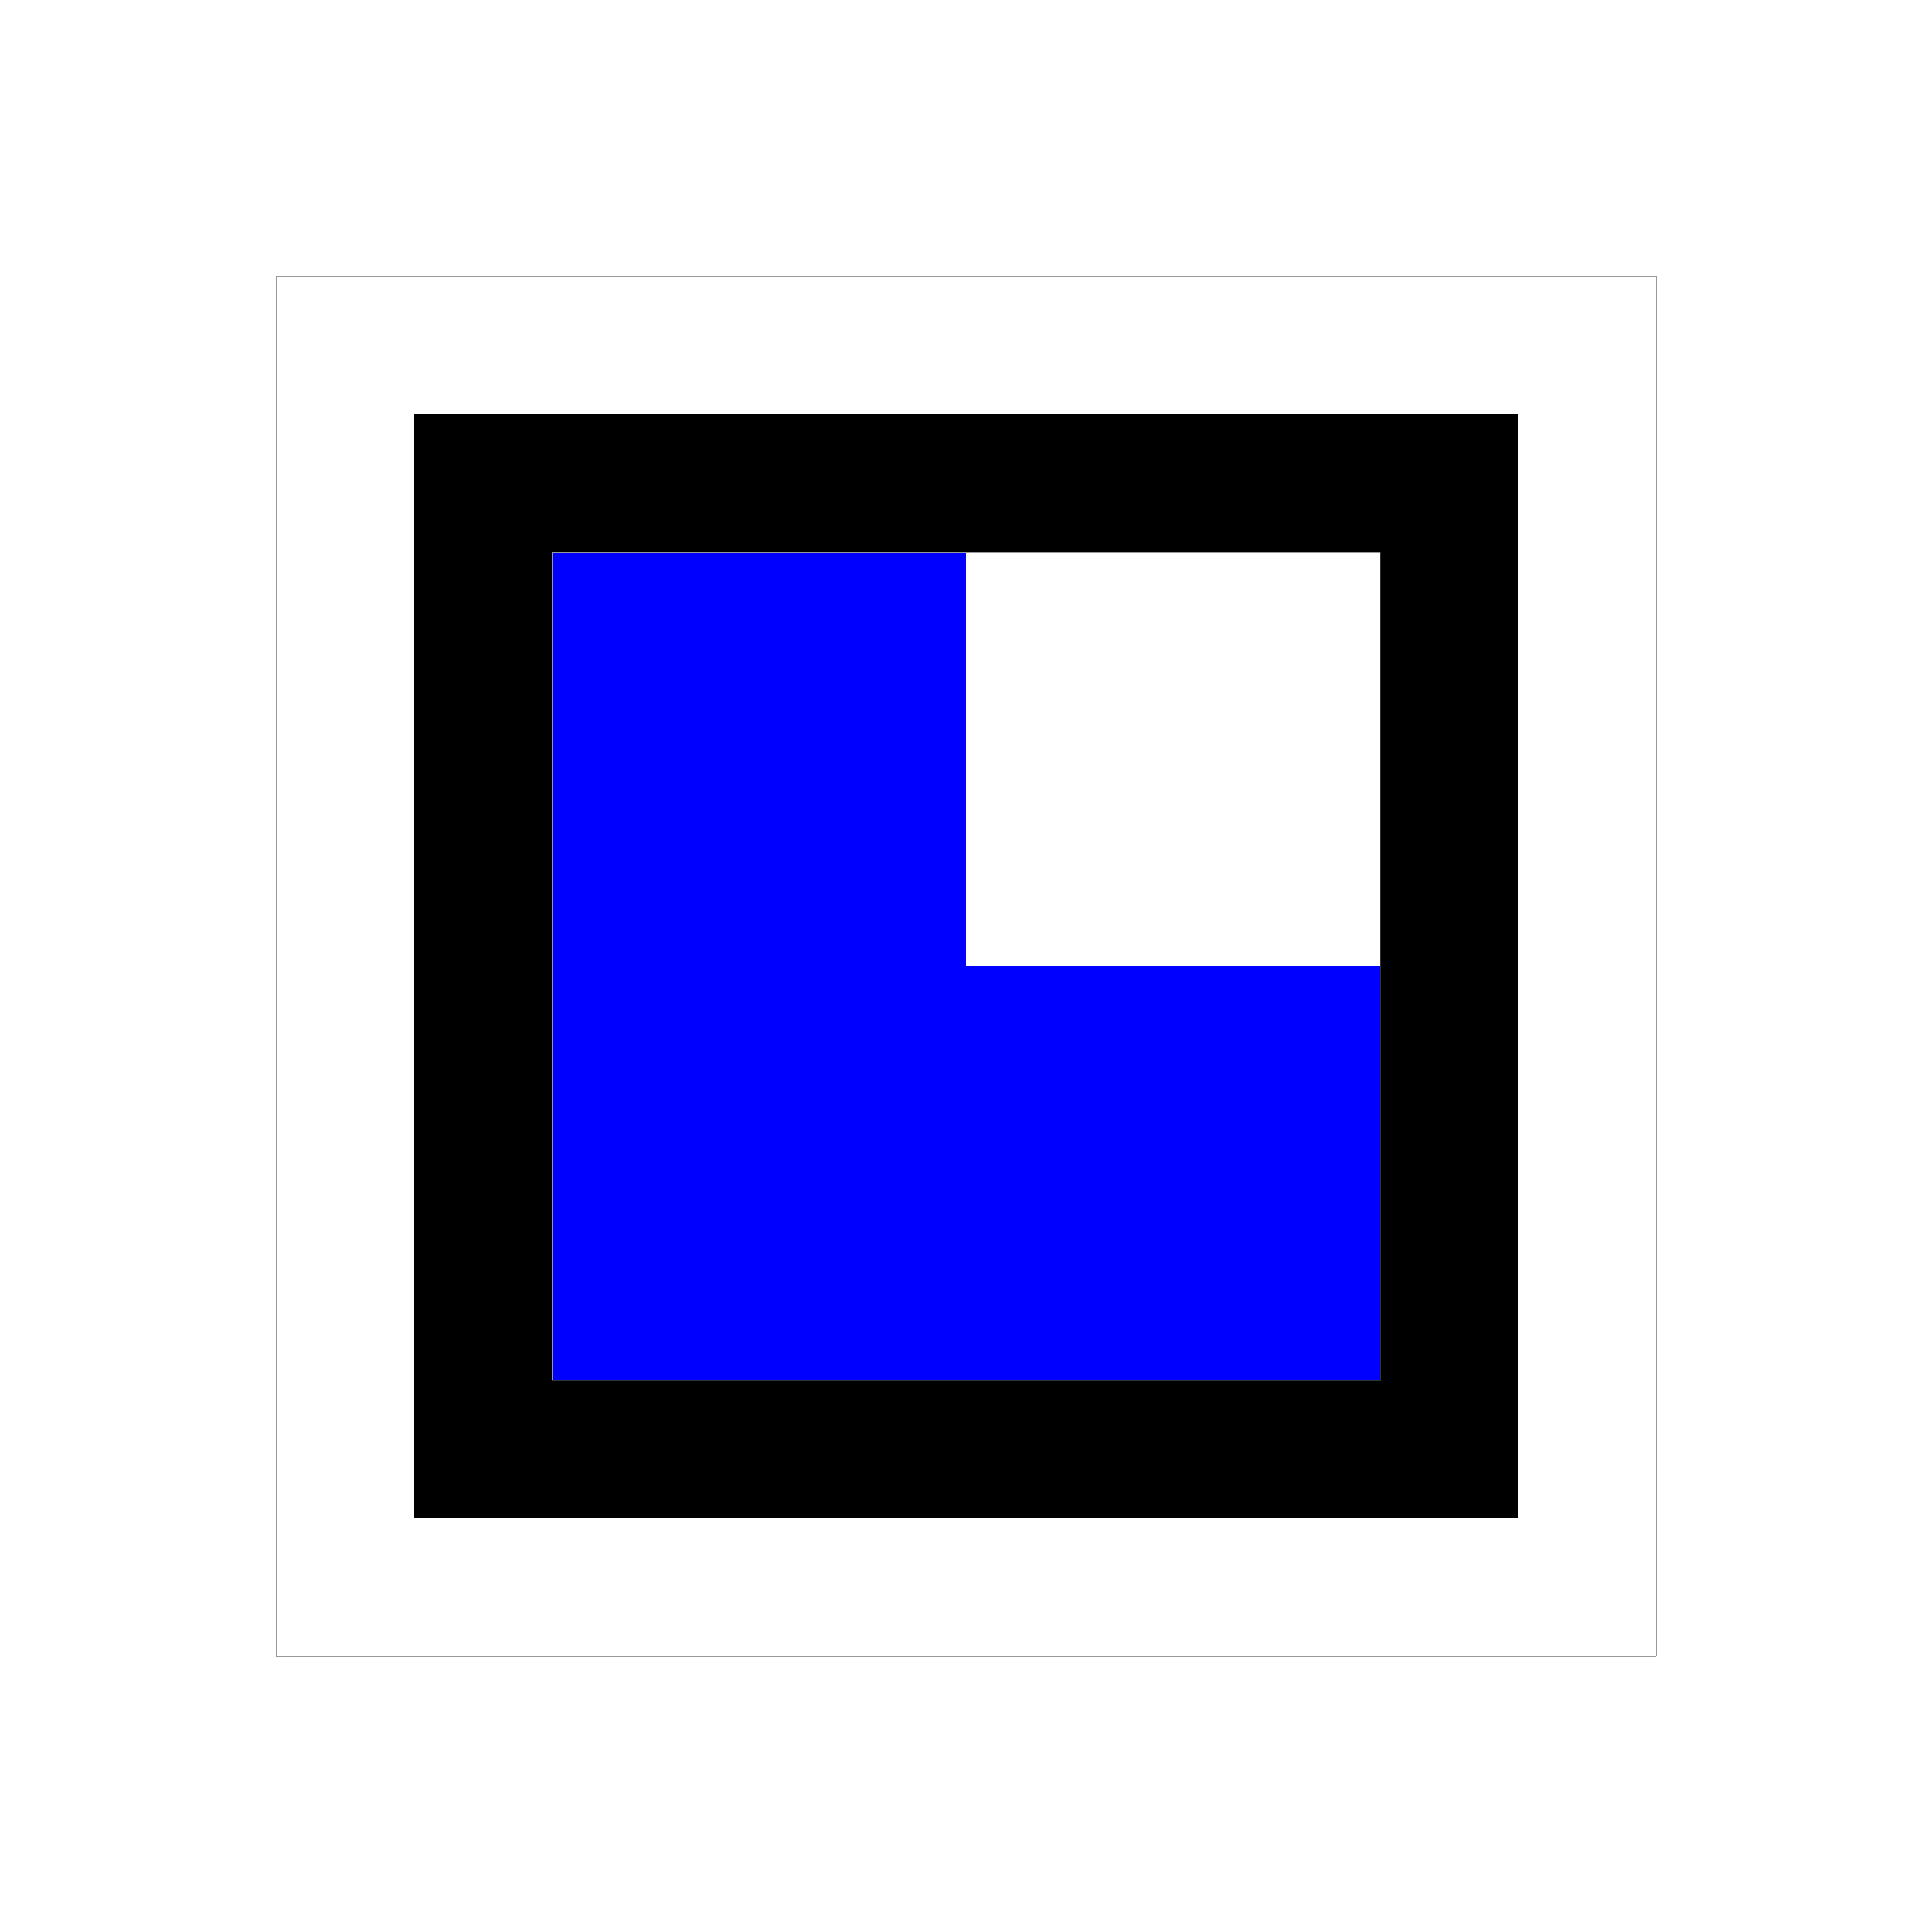
\includegraphics[width=0.17\textwidth]{img/blue}

\includegraphics[width=0.17\textwidth]{img/white}
\includegraphics[width=0.17\textwidth]{img/black}
\caption[다섯 종류의 마커]{다섯 종류의 마커: 왼쪽부터 차례대로 Red, Green, Blue, White, Black.}
\label{img:marker}
\end{figure}


\paragraph{정의된 마커의 종류}
영상 처리 알고리즘에서 가정하는 마커는 그림 \ref{img:marker}에서 나타내는 것과 같이
Red, Green, Blue, White, Black 다섯 종류이다.
이 중 Red, Green, Blue는 식물 살수에서 화분의 종류를 알기기 위해 사용되고,
White, Black은 범위 살수에서 범위의 시작과 끝을 알리기 위해 사용된다.

\paragraph{인식을 위한 마커 규격}
마커는 영상 처리를 통해 인식될 수 있어야 하므로, 아래에서 정의하는 규격에 부합되어야한다.

\subparagraph{부착 형태}
마커의 형태는 정사각형이어야하며, 화분에 부착될 때는 정사각형의 각 변이 지면에 대해 수직 또는 수평을 이루어야 한다.
마커를 인식할 카메라는 지면에 대해 수평한 베이스에 고정되어 팬(좌우 회전) 또는 틸트(상하 회전) 동작을 수행할 수 있다.

\subparagraph{마커 배경}
마커에는 흰색 배경이 아래에서 설명할 테두리의 바깥 방향을 향하여 1cm 이상 할당되어야 한다.

영상 처리를 거쳐 마커를 성공적으로 인식하기 위해서는 배경과 분명히 구별되는 마커의 특성이 있어야 하는데,
흰색 배경을 가정하고 있기 때문에 마커에 흰색 배경을 사용한다.
마커 배경은 마커 규격의 일부분이므로 생략할 수 없으며, 마커 배경이 없거나 장애물이 인식을 방해하는 경우에는
인식률이 현격히 저하될 수 있다.

\subparagraph{테두리}
마커의 네 모서리에 폭 1cm의 흑색 테두리가 할당된다. 흑색 띠의 바깥쪽 경계는 각 변이 8cm인 정사각형,
흑색 띠의 안쪽 경계는 각 변이 6cm인 정사각형을 이룬다.

영상 처리기가 마커로 인지하는 최대 부분은 테두리까지를 포함한다.
따라서 최소한의 마커 배경만을 사용하는 마커 크기는 10cm$\times$10cm이지만,
영상 처리기가 인식하는 테두리만을 포함하는 마커 크기는 8cm$\times$8cm이다.

\subparagraph{색상}
마커 배경과 테두리를 제외한 마커를 4개의 부분 정사각형으로 나누고, 반사율이 낮은 재료\footnote{색종이}를 사용하여
3개의 부분이 특정 색상을 띠도록 해야 한다.

카메라가 인식해야 할 모든 마커 색상의 RGB 채널 속성을 8비트 값으로 나타내면 표 \ref{table:color}와 같다.
마커를 인쇄할 경우에는 CMYK 컬러를 사용하기 때문에 표의 값과 차이가 발생한다.
그렇기 때문에 마커 색상은 인식률이 최대가 되도록 극단적으로 선택된 값으로 되어있다.

\begin{table}[ht]
\centering
\begin{tabular}{c|c|c|c} \hline
마커 색상	& Red	& Green	& Blue	\\ \hline\hline
Red		& 0xFF	& 0x00	& 0x00	\\		
Green	& 0x00	& 0xFF	& 0x00	\\
Blue		& 0x00	& 0x00	& 0xFF	\\
White	& 0xFF	& 0xFF	& 0xFF	\\
Black	& 0x00	& 0x00	& 0x00	\\ \hline

\end{tabular}
\caption{마커 색상에 대응하는 RGB 채널 속성}
\label{table:color}
\end{table}


\paragraph{부가적인 정보 표현}
\label{markerAdd}

\begin{figure}[ht]
\centering
\begin{minipage}{0.17\textwidth}
\subfloat[제1사분면]{
\includegraphics[width=\textwidth,angle=0]{img/green}}
\end{minipage}
\begin{minipage}{0.17\textwidth}
\subfloat[제2사분면]{
\includegraphics[width=\textwidth,angle=90]{img/green}}
\end{minipage}
\begin{minipage}{0.17\textwidth}
\subfloat[제3사분면]{
\includegraphics[width=\textwidth,angle=180]
{img/green}}
\end{minipage}
\begin{minipage}{0.17\textwidth}
\subfloat[제4사분면]{
\includegraphics[width=\textwidth,angle=270]{img/green}}
\end{minipage}

\caption[회전으로 추가 정보 표현]{회전으로 추가 정보 표현: Green 마커가 표현할 수 있는 4가지 상태의 보기.}
\label{img:markerR}
\end{figure}

색으로 구분하는 마커를 추가 개선하는 방법으로, 마커가 부착된 방향에 적은 양의 정보를 추가할 수 있다.
마커는 직교 좌표계에서 원점을 마커의 정 중심으로 보았을 때, 사분면으로 나눌 수 있다.
이 중 3개의 사분면에만 해당하는 색이 칠해지는데, 그림 \ref{img:markerR}과 같이 색이 칠해지지 않은 하나의 사분면의 위치를 인식할 수 있다. 마커의 회전 방향 인식은 PC를 조작하지 않고도 시스템에 간단한 작업을 명령할 수 있게 하는, 이 작품에서 사용된 핵심 기술 중의 하나다.

식물 살수 모드에서는 마커의 방향이 살수 시간 계수를 결정한다.

식물 살수 모드에서, 카메라에서 마커를 바라보았을 때 칠해지지 않은 사분면이
제1사분면인 경우 정상 동작, 제2사분면인 경우 살수 시간을 2배로,
제3사분면인 경우 살수 시간을 $\frac{1}{2}$배로, 제4사분면인 경우 이번 살수 건너뛰기로 명령을 할당한다.

결과적으로 식물의 생육 상태와 주변환경에 따라 살수 시간을 조절하고 싶거나 직접 물을 준 경우에,
사용자는 이 사실을 시스템에 알리기 위해 굳이 딱딱한 키보드를 두드릴 필요가 없다.

범위 살수 모드에서는 마커의 방향이 살수 방식을 결정한다.
행 우선 방식(Row-major order)은 살수 지점을 좌우로 이동하며
전체적으로는 위에서 아래로 쓸어나가는 살수 방식,
열 우선 방식(Column-major order)은 살수 지점을 항상 위에서 아래로 이동하며
전체적으로는 왼쪽에서 오른쪽으로 쓸어나가는 살수 방식,
뒤집힌 열 우선 방식은 살수 지점을 항상 아래에서 위로 이동하며
전체적으로는 왼쪽에서 오른쪽으로 쓸어나가는 살수 방식이다.

상단 1행 살수 기능은 살수 범위의 최상단에만 왼쪽에서 오른쪽으로 살수하는 기능으로,
수압에 의한 청소를 하지 않고 직접 닦아내고자 하는 경우에 유용하다.
범위의 세로 길이가 길어질수록 살수 지점을 느리게 이동하기 때문에,
범위 전체에 물을 빠르게 뿌릴 수 있다.

범위 살수 모드에서, 카메라에서 마커를 바라보았을 때 칠해지지 않은 사분면이
제1사분면인 경우 행 우선 방식 범위 살수,
제2사분면인 경우 열 우선 방식 범위 살수,
제3사분면인 경우 뒤집힌 열 우선 방식 범위 살수,
제4사분면인 경우 상단 1행 살수로 명령을 할당한다.


\subsubsection{이진 인코딩된 마커}

\begin{figure}[ht]
\centering

\includegraphics[width=0.3\textwidth]{img/qrcode}
\caption[QR 코드]{문자열 ``WaterTurret''을 나타내는 QR 코드}
\label{img:qrcode}
\end{figure}

식물 데이터베이스에서 사용할 식물의 수가 3을 초과할 경우에는 마커에 보다 더 많은
정보를 넣기 위해 이진 인코딩된 마커를 사용할 수 있다.

대표적인 예로, ISO 표준으로 공개된 QR 코드가 있다. QR 코드는 빠른 인식 속도와 오류 정정기능,
많은 양의 데이터를 표현할 수 있는 능력이 있어 작품에 응용하기에도 적합하다.
그림 \ref{img:qrcode}은 문자열 ``WaterTurret''을 나타내는 QR 코드인데,
다른 코드에 비해 같은 면적에 많은 양의 정보를 표현할 수 있는 특징을 보여준다.

실제 구현은 식물 데이터베이스에서 엔트리 ID과 같은 화분 정보의 일부를 QR 코드로 직접 인쇄하고 붙이면
적절한 알고리즘을 통해 인식할 수 있다.



\section{작품의 동작 과정}

이 절에서는 동작 과정을 중점으로 작품에 대해 설명한다.
더 자세한 내용은 부록(\ref{appendixHost} 장)에 설명해 두었다.

\subsection{준비}
사용자가 이 시스템을 성공적으로 운용하기 위해서는 일부 설정을 미리 입력해 두어야 한다.

\subsubsection{영상 처리 상수}
영상 처리 과정에서 사용되는 여러 상수는 실험적인 방법을 통하여 최적에 가까운 값을 미리 구해 함께 제공되지만,
표준 마커가 아닌 다른 종류의 마커를 사용하는 경우나 바람이나 광원이 악조건을 형성하는 경우에는
해당 환경에 맞는 상수를 새로 구해야 한다.

\subsubsection{식물 데이터베이스}
식물 데이터베이스는 시스템 운용 중에도 작업에 영향을 미치지 않고 변경할 수 있지만,
시스템에 의해 관리되어야 하는 식물의 종류를 미리 입력해두는 것이 좋다.
식물 데이터베이스에는 인간이 알아볼 수 있는 식물의 이름, 관수 주기, 1회 관수 시간과 같은 정보가 포함된다.

이 시스템을 대규모화할 경우 마커에 이진 인코딩과 같은 방법을 사용해서 많은 정보를 넣을 수 있게 하고
표준화된 식물 데이터베이스를 구축할 수도 있다.

\subsubsection{작동 모드 설정}
시스템을 시작하기 전에 작동 모드를 식물 살수 모드와 범위 살수 모드 중에서 선택해야 한다.
작동 모드는 시스템 운용 중에 수시로 변경할 수 있지만, 한 번에 수행할 수 있는 모드는 오직 하나 뿐이다.
이러한 제한은 제작 과정에 있어서 스케줄링 알고리즘을 단순화하기 위함이다.
두 가지 기능을 동시에 수행해야 하는 경우 이 제한을 제거할 수 있다.

시스템은 각 모드에 대해 잘 정의된 몇 가지 상태 사이를 계속 전이한다.
이러한 상태 사이의 흐름은 시스템이 중지되지 않고 계속 작동하도록 구성되어있다.
시스템이 시작되면 작동 흐름을 \ref{routinePlant}와 \ref{routineRange} 중 하나로 분기하고,
해당 모드의 기본 상태로 진입한다.

\clearpage

\begin{figure}[ht]
\centering
\begin{minipage}{0.34\textwidth}
\subfloat[식물 살수 모드 프로그램 순서도]{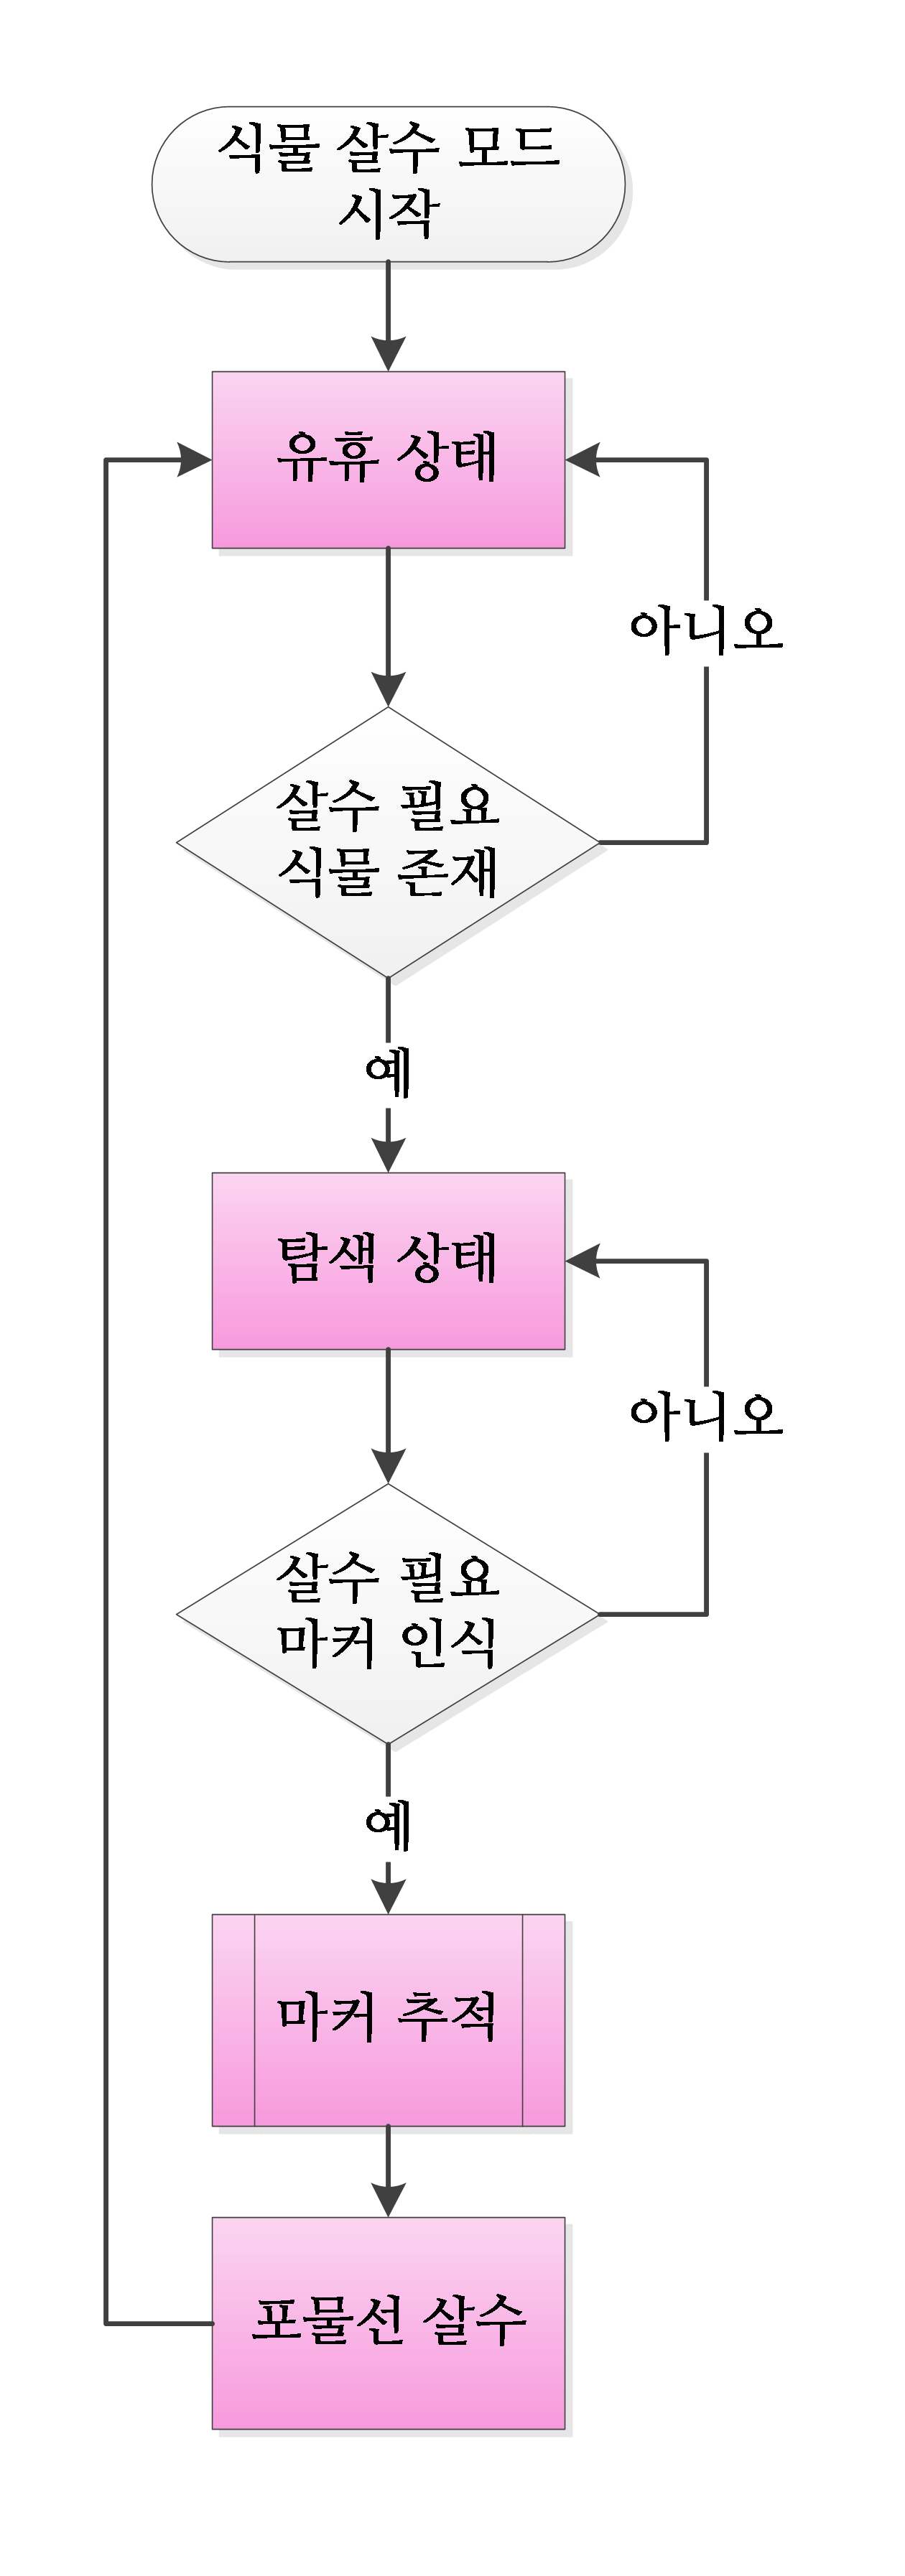
\includegraphics[width=\textwidth]{img/plant}}
\end{minipage}
\begin{minipage}{0.36\textwidth}
\subfloat[범위 살수 모드 프로그램 순서도]{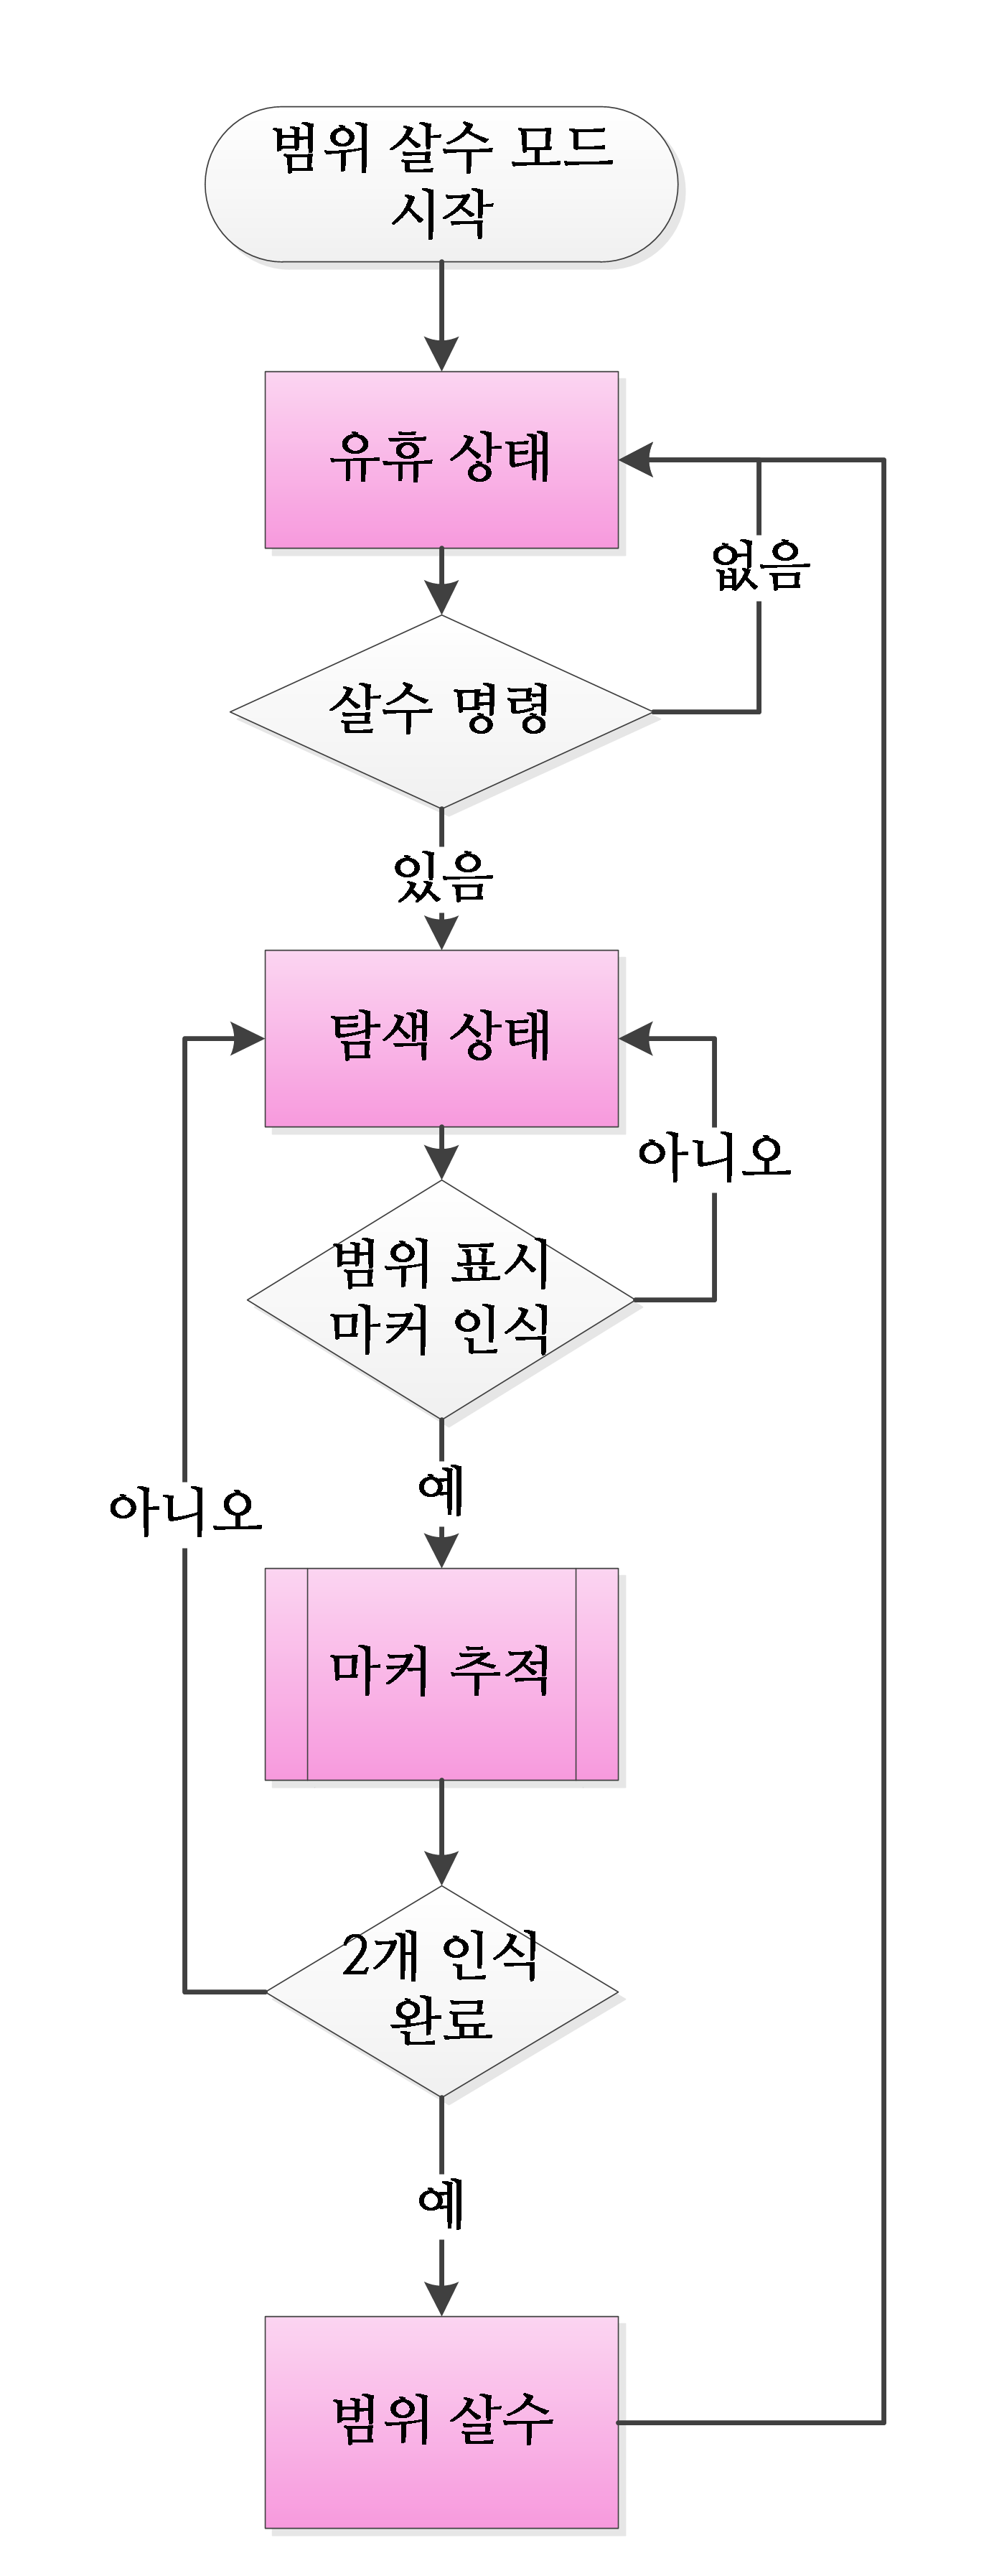
\includegraphics[width=\textwidth]{img/range}}
\end{minipage}

\caption[프로그램 순서도]{프로그램 순서도: 각 모드에서 수행하는 프로그램을 간략화시켜 순서도로 나타내었다.}
\end{figure}



\subsection{식물 살수 모드}
\label{routinePlant}

이 소절은 식물 살수 모드에서의 시스템 동작에 대해 설명한다.
실제 시스템 동작과는 차이가 있으며, 상세한 내용은 부록(\ref{appendixHost} 장)을 참조한다.

\subsubsection{마커 인식과 식물 종류 판단}
식물 데이터베이스에 관수해야 할 식물이 하나 이상 존재하면 시스템이 탐색 상태로 전환되며,
이미지 프로세싱을 통해 카메라 화상에서 마커를 인식한다.
시스템은 인식된 모든 마커에 대해 식물의 종류를 판단하고 관수 필요 여부를 알아낸다.
만약 인식된 마커에 해당하는 식물에 관수가 필요하다면, 다음 단계로 넘어간다.

\subsubsection{마커 추적}
관수가 필요한 식물에 대응되는 마커를 카메라 화상의 중심으로 이동하는 제어를 수행한다.
이 제어가 종료되면 이미지 프로세싱 방법으로 식물과의 거리를 측정한다.

추적이 성공적으로 완료되면 카메라 화상에서 마커가 위치하는 좌표와
카메라와의 거리를 토대로 포물선 살수를 준비한다.

\subsubsection{식물 살수}
식물 데이터베이스에서 정의한 1회 살수 시간동안 펌프를 켜고 밸브를 작동시켜
살수 작업을 진행한다.

\subsubsection{예외 처리}
마커 추적 과정을 진행하는 도중에 추적에 실패하는 것과 같이 시스템 동작 중
예외가 발생할 경우 시스템은 진행 중인 작업을 취소하고 이전 작동 단계로 돌아간다.


\subsection{범위 살수 모드}
\label{routineRange}

이 소절은 범위 살수 모드에서의 시스템 동작에 대해 설명한다.
실제 시스템 동작과는 차이가 있으며, 상세한 내용은 부록(\ref{appendixHost} 장)을 참조한다.

\subsubsection{마커 인식}
범위 살수 모드에서는 직사각형 형태의 범위 전체에 살수할 수 있다.
범위를 표시하기 위한 한 쌍의 마커가 형태 범위의 왼쪽 위와 오른쪽 밑 또는 범위의 오른쪽 위와 왼쪽 밑에 부착된다.

\subsubsection{마커 추적}
마커 하나를 인식할 때 마다 시스템이 마커 추적 상태로 전환된다.
범위를 표시하는 마커를 카메라 화상의 중심으로 이동하는 제어를 수행한다.
이 제어가 종료되면 이미지 프로세싱 방법으로 마커와의 거리를 측정한다.

추적에 성공할 때 마다 상하 / 좌우 제어 정보를 취득하여 위치를 수집한다.
두 마커를 모두 성공적으로 추적했으면 살수를 준비한다.

\subsubsection{범위 살수}
범위의 왼쪽 위와 오른쪽 밑 또는 범위의 오른쪽 위와 왼쪽 밑 정보를 토대로
인식한 범위 전체에 살수 작업을 진행한다.

\subsubsection{예외 처리}
마커 추적 과정을 진행하다가 추적에 실패하는 것과 같이 시스템 동작 중
예외가 발생할 경우 시스템은 진행 중인 작업을 취소하고 이전 작동 단계로 돌아간다.


\chapter{제작 과정}

제작 과정의 위험을 줄이고 완성도 있는 결과물을 얻기 위해
최종 제작품에 이르기까지 총 3차에 걸쳐 작품을 제작, 완성했다.

\section{선행 기술 조사}

KIPRIS를 통해 선행 사례를 조사하였고, 그 내용은 아래와 같다.

\subsection[정원 관리 시스템 및 그 관리 방법]{정원 관리 시스템 및 그 관리 방법 (출원번호 10-2009-0055671)}
요약해보면, 서버에서 작품 생장 환경의 자동 제어를 위한 프로파일을 관리하면서 외부 환경 변화에 따라
제어 장치의 동작을 수행하는 발명이다.

제어 장치의 동작을 자동적으로 제어한다는 점에서는 본 작품과 유사하지만,
본 작품은 영상을 수집함은 물론이고 영상 정보를 적극적으로 활용, 영상 처리를 수행하여 예기치 않게 화분의 위치가
이동된 경우에도 화분의 위치와 종류를 알아낼 수 있다는 점에 크게 구별된다.

\subsection[야생동물 침입 퇴치 장치]{야생동물 침입 퇴치 장치 (출원번호 10-2009-0004114)}
요약하면, 농장에 설치되어 주변 환경을 계속 촬영하다 변화가 감지되면 팬 / 틸트 구동에 의해 물을 투사하여
야생 동물을 퇴치하는 발명이다.

영상 처리를 통해 제어 장치의 작동을 결정하고 물을 투사한다는 점만 유사하며, 식물에 관수하는 부분은 가지고 있지 않다.

\section{1차 제작}

\subsection{주안점}
1차 제작은 장치 제어와 소프트웨어 구조의 안정성을 검증하는 것과,
상하 좌우로 노즐과 카메라를 제어하는 것에 문제가 없는지 알아보는 것에 주안점을 두었다.

\subsection{제작 과정}

\paragraph{팬(좌우) / 틸트(상하) 제어}
장치를 고정할 수 있는 베이스에 좌우 제어를 위한 스테핑 모터를 놓고, 스테핑 모터 구동축 위에
상하 제어를 위한 서보 모터를 고정한다. 서보 모터의 구동축에 적절히 절단된 플라스틱 반찬 용기를 부착한다.

\paragraph{수압 계통}
펌프에서 물이 흡입되는 부분에 호스를 연결해 끝부분이 물통 바닥에 닿도록 넣고,
물이 배출되는 부분은 지름이 더 작은 호스를 사용하고 끝 부분에는 볼펜을 분해해서 얻은 노즐을 끼운다.
플라스틱 반찬 용기에 구멍을 뚫어 노즐을 삽입하고 접착제로 붙인다.

\begin{figure}[ht]
\centering
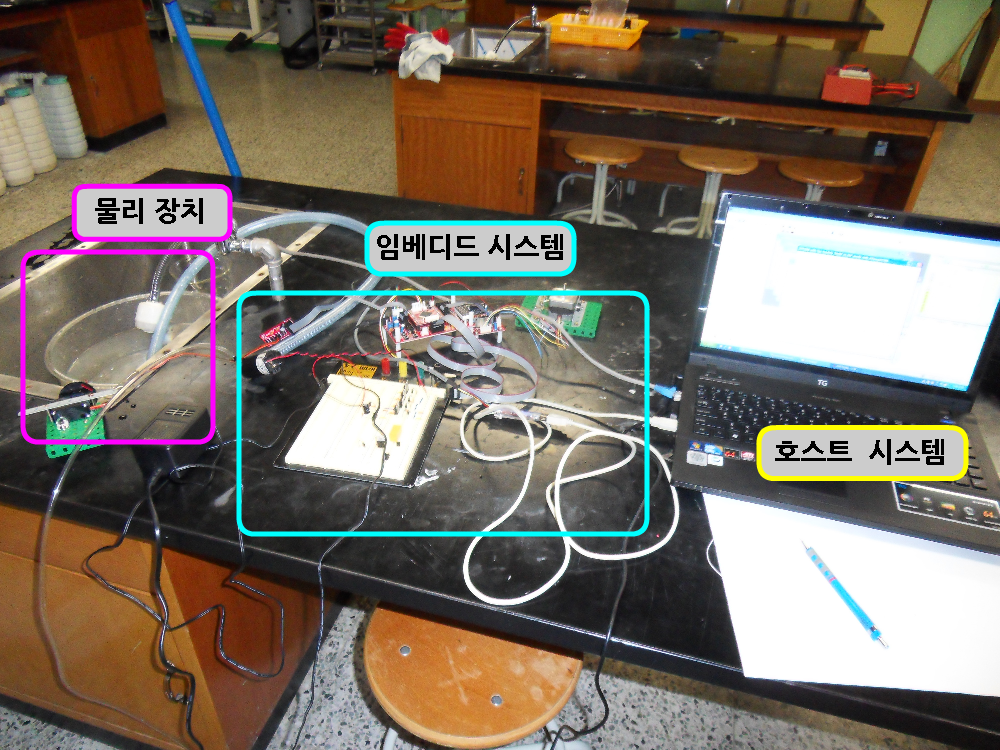
\includegraphics[width=0.70\textwidth]{img/SDC10178}
\caption{1차 제작품의 구조}
\label{img:1a}
\end{figure}

\begin{figure}[ht]
\centering
\includegraphics[width=0.6\textwidth]{img/SDC10189}
\caption{반조립 상태에서 펌프 출력 시험}
\label{img:1b}
\end{figure}

\subsection{제작 결과}

\begin{figure}[ht]
\centering
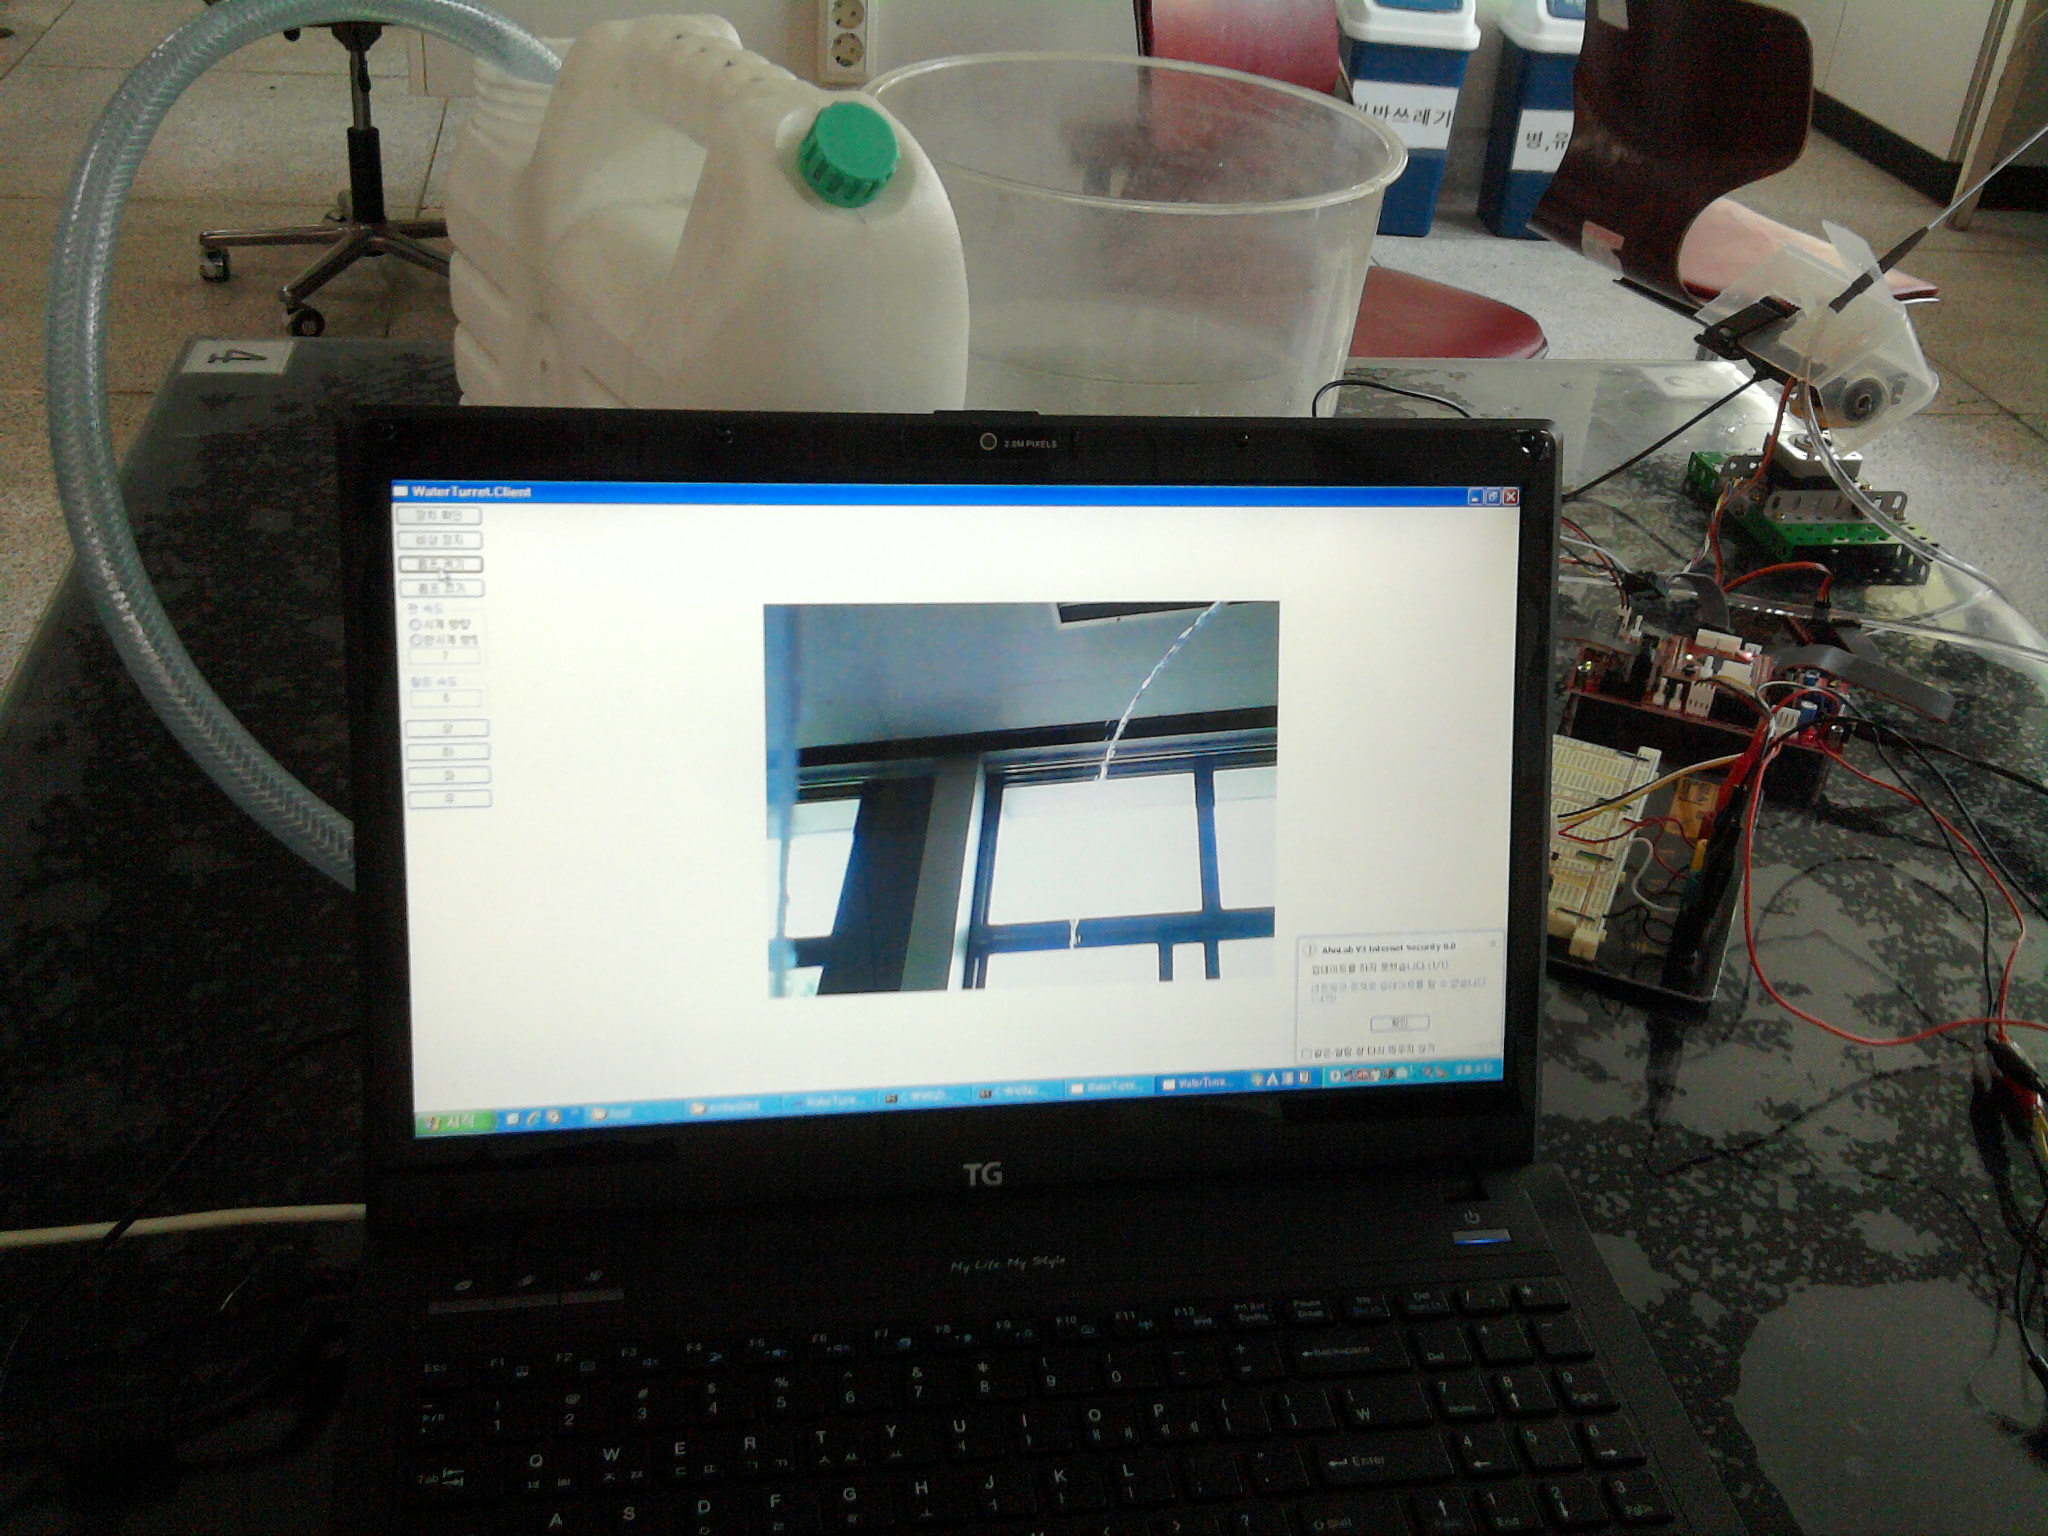
\includegraphics[width=0.6\textwidth]{img/SNC00524}
\caption{1차 제작 완료 시험}
\label{img:1c}
\end{figure}

그림 \ref{img:1c}에서 시험하고 있는 것처럼 1차 제작에서 물을 성공적으로 분사했으나, 물리 장치를 조립하는 부분에서 문제가 있었다.

\paragraph{모터 구동축 축이음}
스테핑 모터의 구동축 지름과 프레임 재료로 사용하고 있는 과학 상자의 축 지름이 각각 5mm와 3mm로, 축을 잇기가 쉽지 않았다.
1차 제작품에서는 이를 나사로 체결하였는데, 축에 대해 수직인 방향으로 힘을 받으면 쉽게 풀려버리는 문제가 있다.

\section{2차 제작}

\subsection{주안점}
2차 제작은 작품에서 핵심적인 기능인 영상 처리 알고리즘과 스케줄러를 개발하고 개선하는 데에 주안점을 두었다.

영상 처리 알고리즘은 카메라를 통해 화분에 부착된 마커를 읽는 역할을 수행한다.
스케줄러는 화분의 상태에 따라 물의 양이나 시간과 같은 한정된 자원을 효율적으로
할당하여 물 공급 계획에 따라 살수하는 역할을 수행한다.

\begin{enumerate}
\item 영상 처리 : 1차 제작에서는 카메라의 영상을 단순히 전송하는 기능만 있었기 때문에
마커 인식은 불가능했다. 영상 처리를 통해 마커를 인식하는 알고리즘을 개발한다.
\item 통신 프로토콜 : 장치에 문제가 있을 때 비상 정지하는 기능에 통신 상의
문제점이 존재하기 때문에 튼튼한 통신 프로토콜을 설계해야 한다.
\item 노즐 각도 제어 : 노즐와 각도가 입력으로 주어졌을 때 노즐 끝을 원하는 각도로 제어할 수 있도록
실제 모터의 회전 각도와 스텝과의 관계를 실험적으로 구하고 테이블을 이용해 직접 사상하거나,
영상 처리를 통한 적응 제어를 구현한다.
\end{enumerate}

1차 제작 시 발생한 기능상의 문제점을 다음과 같이 보완해 보았다.

\begin{enumerate}
\item 전원으로 인한 시스템 불안정성 보완 : 모터 구동용 전원과 신호 전원을 분리하면 전체 시스템을 더 안정적으로 만들 수 있을 것이다.
\item 스테핑 모터 구동축의 불안정성 보완 : 스테핑 모터의 구동축과 과학 상자의 축을 접착제 또는 부드러운 재료로 체결한다.
\end{enumerate}

\clearpage

\subsection{제작 과정}

\paragraph{소프트웨어 개발}
영상 처리 알고리즘과 스케줄러를 개발한다.
그림 \ref{img:test}와 같은 인식 테스트 이미지를 준비하고,
테스트 주도 개발(TDD, Test Driven Development)을 이용해
빠른 속도로 완성도 있는 알고리즘을 개발한다.

\begin{figure}[ht]
\centering
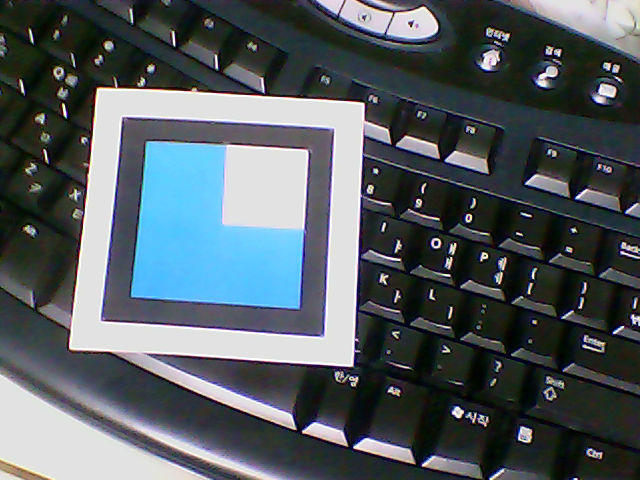
\includegraphics[width=0.45\textwidth]{img/test1}
\hspace{4mm}
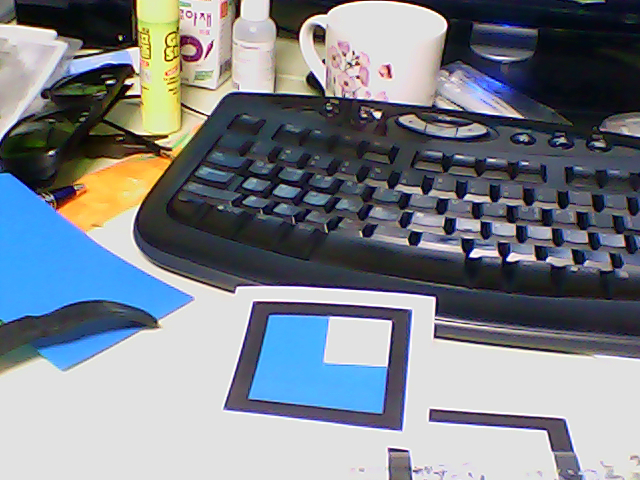
\includegraphics[width=0.45\textwidth]{img/test2}
\caption{인식 테스트 이미지}
\label{img:test}
\end{figure}

\paragraph{전원 분리}
펌프나 밸브가 임베디드 시스템의 불안정적인 동작을 초래할 수 있기 때문에
포토 커플러를 사용하여 전기적으로 절연할 수 있도록 만든다.

\subsection{제작 결과}

\paragraph{전원으로 인한 시스템 불안정성 보완}
임베디드 시스템과 많은 전력을 사용하는 장치의 전원을 분리할 수 있게 되었다.

\paragraph{스테핑 모터 구동축의 불안정성 보완}
접착제와 부드러운 재료를 이용해 축이음을 시도했으나, 높은 회전력을 견디지 못하는 문제점이 발견되었다.
하지만 제작 과정에서, 부품에 구동축와 같은 지름의 천공을 만드는 방법으로 문제를 해결했다.

\begin{figure}[ht]
\centering
\includegraphics[width=0.5\textwidth]{img/SDC10421}
\caption[2차 제작 단계의 임베디드 시스템]{2차 제작 단계의 임베디드 시스템: 사진에는 마이크로 프로세서, 스테핑 모터 제어 모듈, 서보 모터 구동 모듈이 나타나있다.}
\label{img:embedded2}
\end{figure}

\paragraph{소프트웨어 개발}
AForge.NET Framework를 기반으로 하여, 영상 처리 및 스케줄링 소프트웨어를 개발했다. 자세한 내용은 부록(\ref{appendixHost} 장)에서 설명한다.

소프트웨어는 크게 두 부분으로 구성되어 있는데, 영상 처리를 담당하는 부분과
스케줄링 및 관리 기능을 처리하는 부분이다.
영상 처리는 매 프레임 정보가 도착할 때마다 진행하고,
내부 자료구조에 영상 분석 결과를 저장해둔다.
스케줄러는 일정 간격으로 실행하며 이전 실행에서 현재 실행까지의 영상 정보를 토대로
다음 작업 내용을 결정한다. 정보를 시현하는 계층과 작업을 처리하는 계층이 느슨하게 결합된 설계를 사용하기 때문에, 인터페이스나 작업 내용의 변경이 빠르게 이루어질 수 있다.


\paragraph{마커에 추가 정보 포함}

\begin{figure}[ht]
\centering

\includegraphics[width=0.2\textwidth]{img/pYellow}
\hspace{0.4cm}
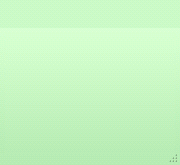
\includegraphics[width=0.2\textwidth]{img/pGreen}
\hspace{0.4cm}

\includegraphics[width=0.2\textwidth]{img/pPurple}

\caption{점착식 메모지로 만든 시험용 마커 (그래픽)}
\label{img:pMarker}
\end{figure}

마커에 특정 색상의 점착식 메모지 또는 점착제가 도포된 재사용 가능한 마커를
원래 마커에 인접하게 부착하여 추가 부착된 마커의 색상에 따라
`정상 살수', `2배 살수', `$\frac{1}{2}$배 살수'와 같이
시스템 동작에 변화를 줄 수 있는 추가 정보가 포함된 마커를 시험해보았다.

그런데 그림 \ref{img:pMarker}과 같은 마커 자체에는 식물의 종류에 대한 정보를
넣을 수 없기 때문에 두 종류의 마커
\footnote{식물의 종류를 나타내는 마커, 추가 정보를 나타내는 마커}를 사용해야 하는데,
좁은 간격으로 화분이 붙어 있거나 마커의 위치가 조금 어긋난 경우
추가 작업을 적용해야 할 식물의 종류를 유일하게 결정하지 못하는 경우가 나타났다.

제작 과정에서 이 같은 문제점을 인지하고,
최종적으로 \ref{marker}와 같이 구현하여 문제점을 해결하였다.



\section{최종 제작}

\subsection{주안점}
최종 제작은 1차 제작과 2차 제작의 문제점을 대부분 보완하면서,
영상 처리에서 거리 측정 구현과 인식률을 향상시키는 데 주안점을 두었다.

\subsection{제작 과정}

\paragraph{듀얼 틸트 제어}
1차와 2차 제작에서 실현하지 못했던 부분으로, 노즐와 카메라를 독립적으로 제어하기 위해
서보 모터를 하나 더 추가한다. 서보 모터를 추가한 배경은 \ref{cam}에서 설명했다.

\begin{figure}[ht]
\centering
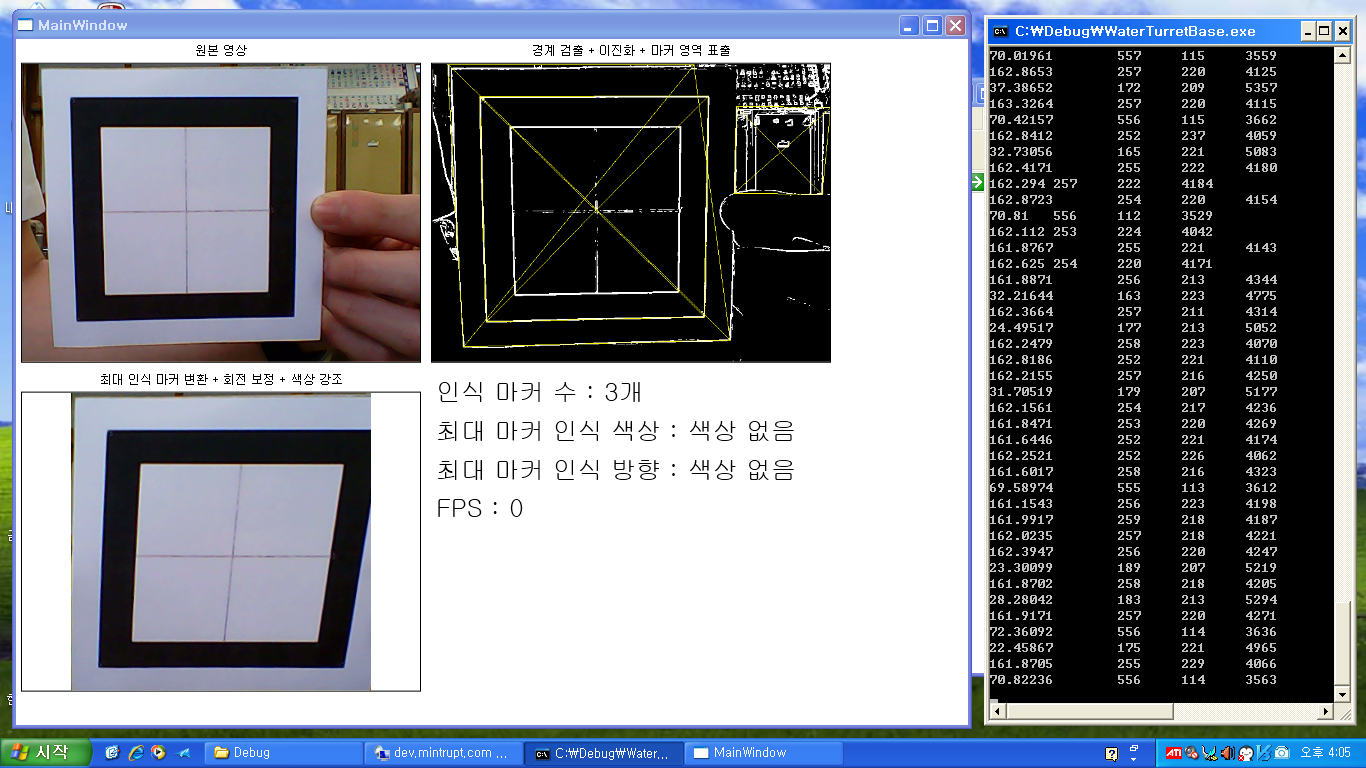
\includegraphics[width=\textwidth]{img/dev}
\caption{영상 처리기 개선 과정}
\label{img:dev}
\end{figure}

\paragraph{영상 처리 개선}
영상 처리를 통해 카메라에서 마커까지의 거리를 측정할 수 있게 하고,
프레임 처리 방식을 개선해 마커를 놓치는 빈도를 줄이도록 처리 방법을 변경한다.
그림 \ref{img:dev}는 영상 처리기를 개선하기 위해 다양한 경우를 테스트하고 있는 모습이다.


\subsection{제작 결과}

\begin{figure}[ht]
\centering
\includegraphics[width=0.6\textwidth]{img/SDC10543}
\caption{최종 제작품의 구조}
% \label{img:}
\end{figure}

\begin{figure}[ht]
\centering
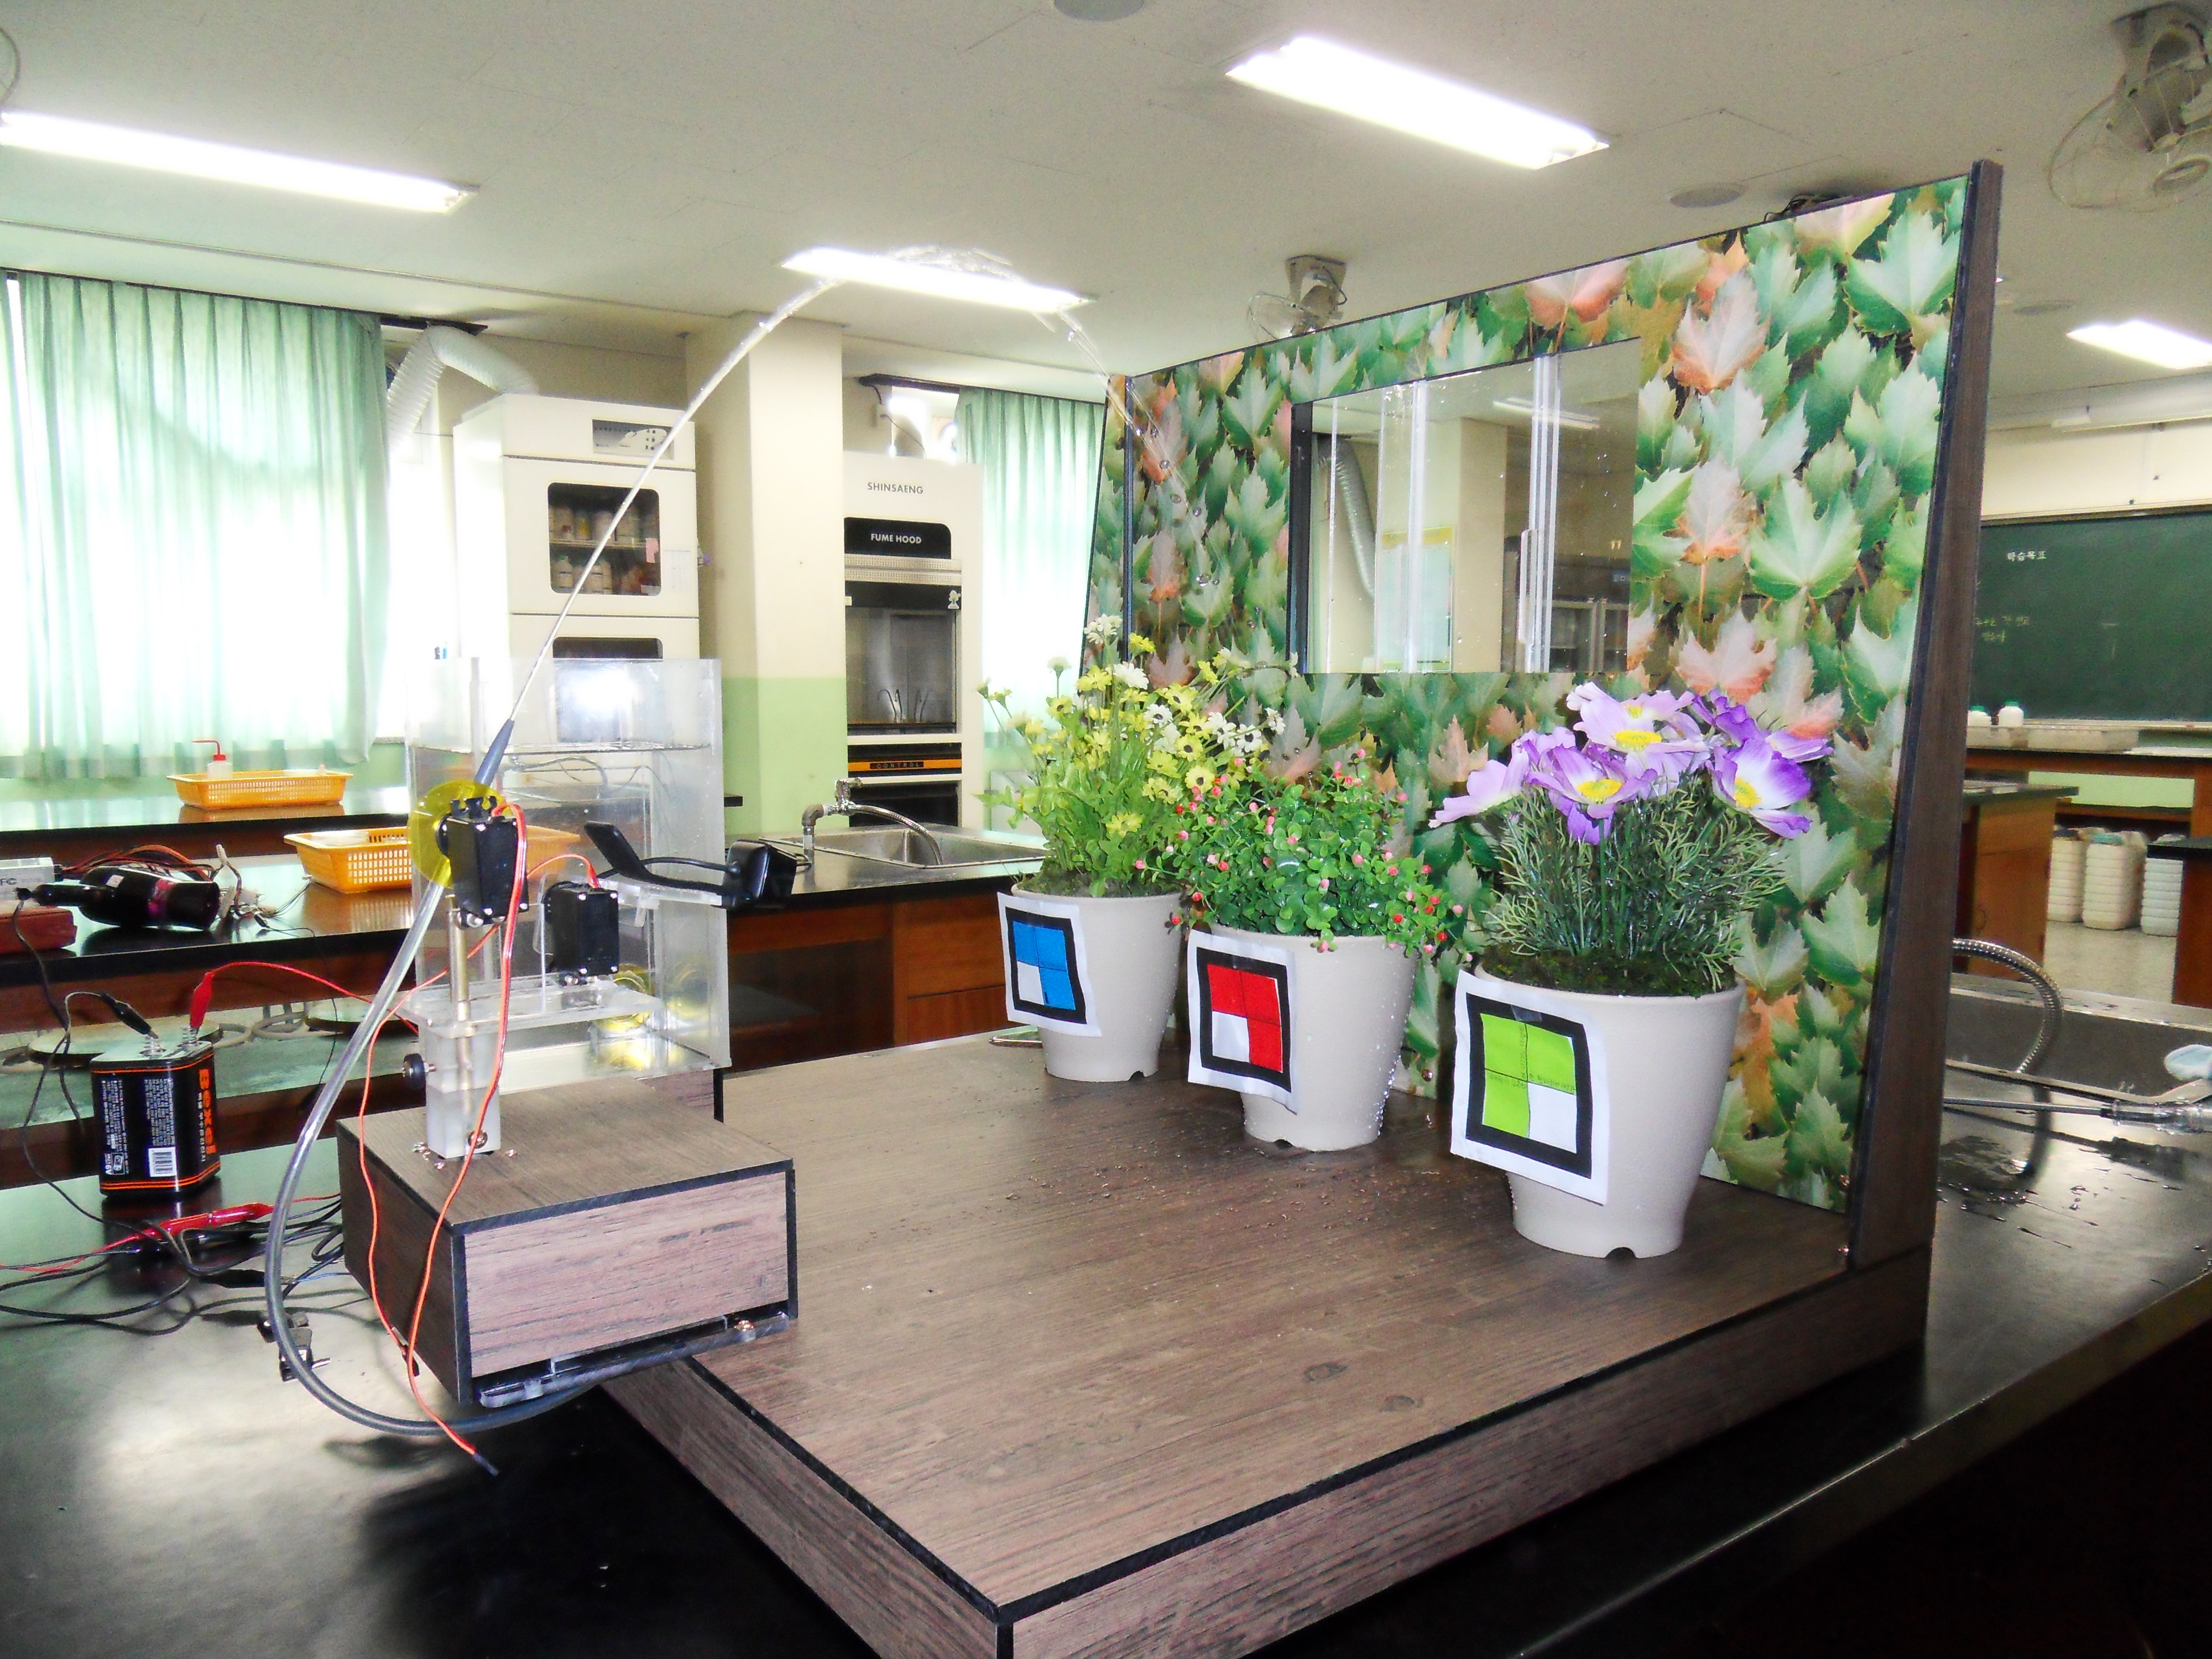
\includegraphics[width=0.6\textwidth]{img/SDC10540}
\caption{최종 제작 살수 시험}
% \label{img:}
\end{figure}

\paragraph{영상 처리를 통한 거리 측정}
마커가 카메라 화상의 중심에 위치하도록 제어했을 때,
화상에서 나타나는 마커의 변형 / 왜곡의 정도를 통해
카메라에서 마커 사이의 거리를 측정할 수 있었다.

\paragraph{영상 처리 인식률 향상}
처리를 진행하는 과정에서 가장 최근 프레임 하나만 탐색하는 방법을 사용하지 않고,
최근의 몇 프레임을 함께 분석하는 방법을 사용한다.
그 결과 추적 과정에서 전체적인 인식률이 향상되어 추적 실패 빈도가 줄어들었다.



\chapter{제작 결과}

\section{작품 제작의 효과}

\subsection{사용자 개입 없이 자동으로 화분을 구별할 수 있었다.}
카메라에서 얻은 화상을 분석하여 화분에 부착된 규격 마커를 추출하고 종류를 인식하여
화분을 구별할 수 있었다.

\subsection{예기치 못한 화분 위치 이동에도 문제 없이 화분을 인식했다.}
실시간으로 매번 전 구역에 대해 영상 처리를 수행할 수 있는 빠른 영상 처리 방법을 개발하여
사용자가 화분을 옮길 때 시스템에 알리지 않아도 화분을 계속 인식할 수 있었다.

\subsection{계획에 따라 스스로 물을 뿌릴 수 있었다.}
식물의 종류와 관수 계획을 미리 등록한 상태에서 영상 처리를 통해
마커까지의 거리를 계산하고 포물선으로 물을 뿌릴 수 있었다.
컴퓨터를 조작하지 않고도 마커의 회전 각도만을 변화시키는 방법으로 관수 계획에 유연한 변화를 만들 수 있었다.

\subsection{사용자가 수동으로 실시간 제어할 수 있었다.}
사용자가 원하는 경우 시스템의 작동을 중지하고 직접 실시간으로 제어할 수 있었다.
추후 원격 실시간 제어로 쉽게 확장할 수 있도록 설계하였다.

\subsection{마커로 특정 범위를 표시하고 범위 내부에 물을 분사할 수 있다.}
사용자가 직접 한 쌍의 마커로 범위를 표시하면 시스템이 두 마커를 인식하고 범위를 계산하여
사용자가 표시한 범위 전체에 물을 분사할 수 있었다.

\section{개선 방안}

\subsection{인식 가능한 식물 마커의 수 개선}
화분에 부착할 수 있는 마커가 세 종류로 매우 제한적이다.
마커 규격에 앞서 언급한 이진 인코딩을 반영하여 많은 수의 마커를 인식할 수 있도록 개선할 수 있다.

\subsection{다양한 자동 제어 기능 추가}
식물 생육을 자동 관리하기 위해서는 수분 관리 뿐만 아니라 온도, 습도, 빛과 같은 다양한 요소를
다룰 수 있어야 한다. 여러가지 종류의 센서를 추가하고 항온항습기나 조명 장치 등과 연동할 수 있도록 하면
사용자의 개입을 더 줄일 수 있을 것이다.

\section{향후 전망}
카메라는 사용자가 보유한 일반적인 USB 웹캠을 부착하여 사용할 수 있고,
마커는 일반적인 컬러 프린터로 쉽게 인쇄할 수 있으며,
시스템을 운용하기 위해 고사양의 PC가 필요하지 않다.
따라서 가정에 시스템을 도입하는 데 있어 큰 부담이 없을 것으로 생각된다.

식물 살수 기능은 교실, 가정의 베란다, 건물 옥상에서 유용하게 사용될 것이고,
범위 살수 기능은 창문의 윗 부분이나 방충망, 천장, 간판 청소와 같이
더럽거나 높은 조건 때문에 사람이 접근하기 힘든 경우에 무리 없이 적용될 것이다.


% \begin{thebibliography}{99}
% \end{thebibliography}



\chapter{부록}
\label{appendixHost}

\appendix

\section{Context}
호스트 시스템은 전체적으로 하나의 문맥 개체를 유지한다.
시스템은 문맥의 상태에 따라 일관된 동작을 수행하며, 문맥 상태를 계속 전이시키며 작동한다. 문맥에는 세 가지의 모드가 있다. None은 작업이 없는 상태,
Plant는 식물 살수 모드, Range는 범위 살수 모드이다.

다음은 식물 살수 모드에서의 상태 목록이다.
\begin{itemize}
\item Idle : 작업을 시작하지 않았거나 살수할 필요가 없어 작동하지 않는 상태입니다.

모드에 처음으로 진입할 때 설정된다. Idle 상태에서는 명확하게 살수할 필요가 없는 경우를 제외하고 항상
다른 상태로 전환하기 때문에 다른 상태에서 예외가 발생하거나 작업을 완료한 경우에는 항상 이 상태로 전이한다.

Idle 상태에서 살수가 필요하지 않은 경우란, 식물 데이터베이스에 포함된 모든 식물의 살수가 필요 없는 경우이다.

\item Searching : 살수가 필요한 식물을 찾고 있습니다.

살수가 필요한 식물이 하나 이상 존재하는 상태이다. 이 상태에서 마커를 인식하면 마커가 대응되는 식물의
살수 요구 여부를 확인하고, 필요하다면 Tracking 모드로 전이한다.

\item Tracking : 살수가 필요한 식물을 찾았고 추적을 시도하고 있습니다.

식물에 해당되는 마커를 계속 추적하여 카메라 화상의 중앙에 오도록 제어한다.
이동 과정에서는 흔들린 화상에 의해 인식률이 떨어지기 때문에 짧은 시간 동안 마커 인식에 실패할 수 있다.
하지만 일시적인 인식 실패가 아닌 장애물과 같은 다른 원인이 있을 수 있기 때문에
마커를 잃어버린 시간이 미리 설정한 임계 시간보다 커지면 추적을 포기하고 Idle 상태로 전이한다.

추적에 성공한 경우, 마커와의 거리를 측정하고 노즐 각도를 수정한 후, Watering 상태로 전이한다.

\item Watring : 추적이 완료되어 살수 중입니다.

살수가 필요한 시간 동안 펌프를 켜고 밸브를 개방하여 살수 작업을 진행한다.
요구 시간 이상 살수한 경우 펌프와 밸브를 정리한 다음 Idle 모드로 전이한다.

\item Manuel : 수동으로 작동 중입니다.
\end{itemize}

다음은 범위 살수 모드에서의 상태 목록이다.
\begin{itemize}
\item Idle : 작업을 시작하지 않았거나 살수할 필요가 없어 작동하지 않는 상태입니다.

범위 살수 모드에서는 사용자 요구 없이 작업을 시작하지 않는다. 만일 사용자 요구가 있는 경우에는
두 마커를 모두 찾지 못했을 때 Searching 상태, 두 마커를 모두 찾았을 때 Watring 상태로 전이한다.

만약 사용자가 작업을 중지한 경우에는 두 마커의 정보와 같은 변수를 모두 초기 상태로
되돌린다.

\item Searching : 살수가 필요한 범위를 나타내는 두 마커를 탐색 중입니다.

\item Tracking : 범위 마커를 찾았고 추적을 시도하고 있습니다.

마커를 계속 추적하여 카메라 화상의 중앙에 오도록 제어한다.
이동 과정에서는 흔들린 화상에 의해 인식률이 떨어지기 때문에 짧은 시간 동안 마커 인식에 실패할 수 있다.
하지만 일시적인 인식 실패가 아닌 장애물과 같은 다른 원인이 있을 수 있기 때문에
마커를 잃어버린 시간이 미리 설정한 임계 시간보다 커지면 추적을 포기하고 Idle 상태로 전이한다.

추적에 성공한 경우, 마커와의 거리를 측정하고, 결과를 저장한다.
저장된 마커의 수가 2개인 경우에는 마커가 왼쪽 위와 오른쪽 아래 또는 오른쪽 위와
왼쪽 아래 중 어떤 지점을 나타내는 지 판단한 후, Watering 상태로 전이한다.

\item Watering : 살수 범위에 자동 살수하고 있습니다.

\ref{markerAdd}에서 설명한 살수 방식에 따라 살수를 진행하게 된다.

\item Manuel : 수동으로 작동 중입니다.

식물 살수 모드에서의 Manuel 상태와 다른 점은, 식물 마커에 대한 시각화가 제공되지 않는다는 것이다.

\end{itemize}

\section{ImageProcessor}

영상 처리는 AForge.NET Framework를 기반으로 한다. 영상 처리는 다음과 같은 과정으로 이루어진다.

\begin{enumerate}

\item BT709 알고리즘에 의해 그레이스케일 영상을 얻는다.

\item 에지 검출기가 그레이스케일 영상에서 경계를 검출한다.

\item 미리 설정한 임계값을 기준으로 경계 검출 영상을 이진화한다.

\item 이진화된 영상에 세그멘테이션과 라벨링을 수행하여 이미지를 작은 부분으로 나누고 마커 후보에 추가한다.

\item 미리 설정한 값을 바탕으로 각각의 마커 후보가 적합한지 검사한다.
마커가 사각형 형태인지, 사각형일 경우 각 변이 이루는 각이 허용치 이내인지,
각 변 사이의 비율이 허용치 이내인지, 명확한 검정색 테두리를 가지고 있는지 검사한다.
모든 검사를 통과한 후보를 마커로 최종 인식한다.

\item 화상에 위치한 마커의 무게 중심을 구해 화상 중심을 원점으로 하는 마커 좌표를 결정한다.

\item 마커의 꼭짓점의 좌표의 순서를 수정하여 방향을 보정한다.

\item 변형된 마커의 방향과 길이 왜곡을 보정하여 정사각형 이미지로 변환한다.

\item 마커의 색상을 판정한다. Red, Green, Blue 각 채널에 대해 히스토그램 중간값을 구하고
미리 설정한 값을 바탕으로 가장 우세한 채널을 선택한다.
가장 강도가 높은 채널과 두 번째로 강도가 높은 채널과의 차이가 너무 적은 경우에는
마커 색상을 White, Black 중 하나로 결정한다.

\item 마커 색상이 Red, Green, Blue, Black 중 하나로 결정된 경우 회전 판정을 수행한다.
회전 판정은 먼저 마커의 그레이스케일 영상을 얻고 4개의 사분면으로 분할한다.
각 사분면 데이터에서 평균값을 구하고, 다른 사분면과 비교해 하나의 사분면을 찾는다.

\end{enumerate}

\end{document}
